 \documentclass[a4paper,10pt]{article}
\usepackage[utf8]{inputenc}
\usepackage[spanish]{babel}
\usepackage[affil-it]{authblk}
\usepackage{enumerate}
\usepackage{graphicx}
\usepackage{hyperref}
\usepackage{amsmath}
\usepackage{amssymb}
\usepackage{array}
\usepackage{cancel}
\usepackage[usenames, dvipsnames]{color}
\usepackage{tikz}
\usepackage[labelfont=bf]{caption}
\usepackage{subcaption} %Multiple images
\usepackage{multicol} % Multiple columns
\usepackage{float}
\usepackage{cleveref}
 \usepackage{relsize} % bigger math symbols
\usepackage[margin=1.4in]{geometry}
\usepackage[titletoc,toc,title]{appendix}
\usepackage{enumitem}
\usepackage{etoolbox}
\usepackage{authblk} %multiple authors
\usetikzlibrary{calc}
\numberwithin{equation}{section}

% Center values table
\newcolumntype{P}[1]{>{\centering\arraybackslash}p{#1}}

% Circled words
\newcommand{\circled}[2][]{%
  \tikz[baseline=(char.base)]{%
    \node[shape = circle, draw, inner sep = 1pt]
    (char) {\phantom{\ifblank{#1}{#2}{#1}}};%
    \node at (char.center) {\makebox[0pt][c]{#2}};}}
\robustify{\circled}

%Appendices in spanish
\renewcommand{\appendixname}{Ap\'endices}
\renewcommand{\appendixtocname}{Ap\'endices}
\renewcommand{\appendixpagename}{Ap\'endices}

%Zero delimiter
\newcommand{\zerodel}{.\kern-\nulldelimiterspace}

%Columns separation
\setlength{\columnsep}{1cm}

%Indentation
\setlength{\parindent}{0ex}

%Multiple References

\crefrangelabelformat{equation}{(#3#1#4--#5\crefstripprefix{#1}{#2}#6)}

\usepackage{xparse}

%Boxes

\newcommand*{\boxcolor}{blue}
\makeatletter
\renewcommand{\boxed}[1]{\textcolor{\boxcolor}{%
\tikz[baseline={([yshift=-1ex]current bounding box.center)}] \node [rectangle, minimum width=1ex,rounded corners,draw] {\normalcolor\m@th$\displaystyle#1$};}}
 \makeatother

%Constantes
\newcommand{\euler}{\mathrm{e}}
\newcommand{\im}{i}

% Definición de las secciones y su numeración

\makeatletter
\def\@seccntformat#1{%
  \expandafter\ifx\csname c@#1\endcsname\c@section\else
  \csname the#1\endcsname\quad
  \fi}
\makeatother

%opening
\title{{\huge Sobre el detector BATATA} \\
\vspace{.2cm}
\large Laboratorio Avanzado - Detección de Rayos Cósmicos}

\author[1]{Favio Vázquez\footnote{\url{favio.vazquezp@gmail.com}}}
\author[2]{Susana Marín\footnote{\url{susyma3005@gmail.com}}}
\author[1]{Francisco Huante \footnote{\url{francisco.huante@correo.nucleares.unam.mx}}}
\author[3]{Antonio Rojas \footnote{\url{tinyplack@gmail.com}}}

\affil[1]{Instituto de Ciencias Nucleares,
Universidad Nacional Autónoma de México}
\affil[2]{Instituto de Química,
Universidad Nacional Autónoma de México}
\affil[3]{Instituto de Física,
Universidad Nacional Autónoma de México}

\date{}

\begin{document}

\maketitle

\section{Discusión del detector}

\subsection{Geometría del detector}

BATATA (Buried Array Telescope at Auger) es un detector prototipo que se añadió 
a AMIGA para cuantificar la contaminación electromagnética, y medir el radio entre
la componente muónica y electromagnética proveniente de las lluvias de rayos cósmicos 
como una función de la profundidad subterránea. El detector se instaló en el 
arreglo AMIGA y se seleccionaron lluvias de aire extensas de alrededor de 10 PeV 
con un arreglo triangular de 200 m de lado compuesto con estaciones Cherenkov
de superficie 3+2 de Auger.

\vspace{.3cm}

El detector está compuesto por tres planos de doble capa horizontales enterrados 
a diferentes profundidades. Cada capa en un plano consiste en 49 tiras rectangulares 
de 2 m de largo, 4 cm de ancho y un 1 cm de grosor. Las dos capas del plano están 
rotadas $90^\circ$ para producir un plano $x-y$ efectivo con $4.1$ cm $\times 4$ cm 
píxeles cubriendo un área de $4$m$^2$. Cada plano $x-y$ está adentro de una cubierta 
hecha de fibra de vidrio. Dos tapas permiten el acceso a las tarjetas del ``front-end'' 
y los acoplamientos entre los tubos fotomultiplicadores y las galletas de fibra 
óptica. Las tapas pueden ser desmontadas para inspección y servicio. Más aún, las 
cubiertas y tapas son lo suficientemente versátiles para permitir la adición de 
nuevos componentes y cableados no especificados en el diseño original. El consumo 
de potencia de BATATA es menor que 200 W. Ésta es suministrada por un arreglo 
de 20 paneles solares con sus correspondientes baterías, que aseguran una operación 
continua aún en los meses de invierno donde no hay mucho sol. 

Debajo se muestran algunas imágenes de la geometría del detector,

\begin{figure}[H]
 \center 
 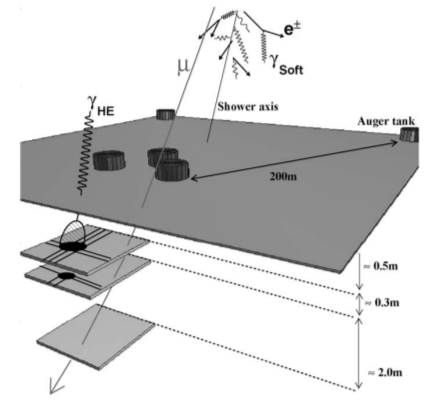
\includegraphics[scale=0.5]{fig1}
 \caption{Tanques tipo Auger en la superficie y centelladores de plásticos del 
 detector y su principio de trabajo. Tomada de \cite{alfaro}.}
\end{figure}

\begin{figure}[H]
 \center 
 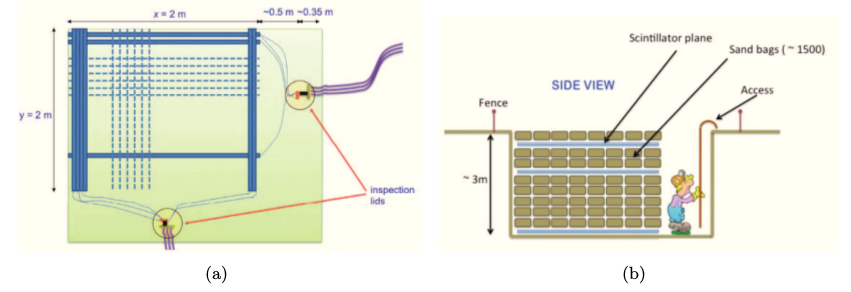
\includegraphics[scale=0.46]{fig2}
 \caption{(a) Vista esquemática de la disposición de los centelladores, 
 fibras ópticas, tubos fotomultiplicadores y electrónica de front-end adentro 
 de la cubierta de cualquiera de los tres planos del detector. (b) Vista lateral 
 esquemática de la disposición del detector. Tomada de \cite{trovato}.}
\end{figure}

\subsection{El centellador}

Los centelladores sólidos han sido utilizados extensivamente en los detectores 
de física de partículas, y en particular estos han sido los detectores preferidos 
para calorímetros de muestreo. Algunas características fueron requeridas para 
los centelladores que se utilizaron en la construcción de BATATA, entre ellas: 

\begin{itemize}
 \item \underline{Buena resolución energética}: La salida de luz debía ser suficiente 
 para que la eficiencia de detección para los muones cruzando una tira fuera mayor 
 a 90\%. 
 \item \underline{Uniformidad}: Para asegurar que era posible corregir para la dependencia 
 de posición de los eventos de lluvia, la salida de luz de las tiras centelladoras 
 no debía variar más de 30\% con respecto a la respuesta nominal a esa posición. 
 \item \underline{Atenuación}: La luz observada desde los lados cercanos y lejanos 
 de las tiras no debía diferir más que un factor de 5.
 \item \underline{Temporización rápida}: Los detectores de centelleo debían tener 
 propiedades intrínsecas que permitieran temporización en nanosegundos.
 \item \underline{Flexibilidad en la lectura de salida.}
 \item \underline{Construcción simple y robusta}: Que el ensamblado de las tiras 
 de centellador sólidas en los módulos del detector requiriera poco hardware y 
 experiencia.
 \item \underline{Estabilidad a largo plazo}: La salida de luz del sistema centellador 
 debía tener una estabilidad a largo plazo con un tiempo de decaimiento de al menos 
 10 años.
 \item \underline{Bajo mantenimiento}: El sistema debía ser bastante robusto y requerir 
 bajo mantenimiento.
 \item \underline{Confiabilidad}: No deberían existir fallas en los centelladores 
 que no puedan ser reparados externamente. Se debería poder corregir el decrecimiento 
 en la salida de luz usando datos de calibración. 
\end{itemize}

Las tiras centelladoras son tipo MINOS \cite{minos}. Están hechos de poliestireno, 
dopados con los flúor PPO (1\%) y POPOP (0.030\%). Este compuesto es derretido y 
extruido en la forma de una barra rectangular con una ranura angosta a lo largo del 
centro de uno de los lados anchos. La profundidad de la ranura es lo suficiente 
para contener una fibra óptica de 1.5 mm de diámetro. Una fina capa exterior de 
TiO$_2$ (0.25 mm) recubre la barra centelladora casi totalmente excepto por una 
pequeña región cerca de la ranura y los extremos laterales, para prevenir que luz 
escape y se incremente la probabilidad de captura por la fibra óptica. Cada tira 
de centellador tiene 4.1 cm de ancho, 1 cm de grosor y 2 m de largo.

\begin{figure}[H]
 \center 
 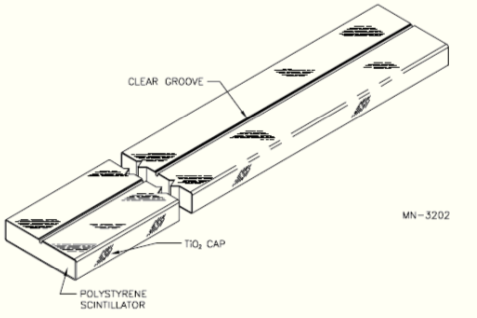
\includegraphics[scale=0.5]{fig3}
 \caption{Vista esquemática de una tira centelladora con ranura y cobertura 
 reflectiva. Tomada de \cite{trovato}.}
\end{figure}

\subsection{Fibra óptica}

Para garantizar una salida de luz aceptable, las fibras ópticas producidas por 
Bicron y Kuraray fueron probadas en el laboratorio. Se escogió para el detector 
una fibra óptica de desplazamiento de longitud de onda (WLS\footnote{Wavelength 
shifting fibers.} en inglés). Cuando una partícula cargada viaja a través de la 
barra centelladora, una fracción de la luz producida es colectada por la fibra 
óptica y re-emitida a una longitud de onda diferente. Cada una de las capas $x$ 
o $y$ de BATATA necesita al menos 141.4 m de fibra óptica, por lo tanto el requerimiento 
total de fibra óptica del detector es de 848-4 m.

\vspace{.3cm}

El acoplado de la fibra óptica al tubo fotomultiplicador requiere de un pulido 
muy fino de la superficie que toca el vidrio en el final del fotocátodo. Para este 
propósito se usó un cuchillo de hojilla que proveyera un corte eficiente, y se necesitó 
mucho cuidado para evitar que se rompieran las fibras. Luego del cortado se 
requirió un fino pulido para asegurar una punta plana y perpendicular al eje de 
la fibra. Este paso fue muy importante debido a que una punta inclinada o sucia 
no puede ser acoplada al tubo fotomultiplicador sin que resulte en una considerable 
pérdida de luz. Se hicieron muchas pruebas para determinar el buen funcionamiento de 
las fibras, y se limpiaron un pulieron las fibras por última vez para asegurar una 
buena conexión con los tubos fotomultiplicadores. Debajo se muestran las puntas de 
las fibras luego de cada etapa. 

\begin{figure}[H]
 \center 
 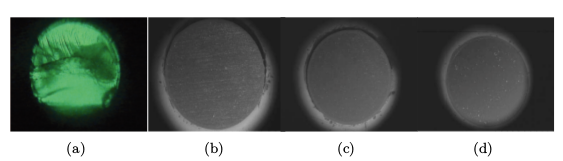
\includegraphics[scale=0.7]{fig4}
 \caption{Vista frontal de una fibra obtenida con un microscopio electrónico para 
 los diferentes pasos del pulido. (a) luego del cortado; (b) luego del pulido con una 
 lija de 2000-grit; (c) luego del pulido con una lija de 3 $\mu$m; (d) luego de un segundo 
 pulido con una lija de 3 $\mu$m. Tomada de \cite{trovato}.}
\end{figure}

\subsection{Electrónica}

La luz de centellador proveniente de cada capa es colectada por un tubo fotomultiplicador 
de 64 píxeles (H7546B). La electrónica funciona en modo de contador y las señales 
son transmitidas a la superficie de la etapa de adquisición de datos usando una 
señalización diferencial de bajo voltaje. Una señal lógica es producida solo 
cuando la altura del pulso analógico es mayor que un umbral dado, y los umbrales 
de cada canal puede ser ajustado independientemente a tiempo real. Cualquier señal 
sobre el umbral abre una ventana de colección de datos de 2 $\mu$s GPS. Los datos, 
incluyendo la señal y el fondo, se adquieren con un sistema de tajetas FPGA Spartan 
y una computadora TS7800 de una sola tarjeta. El código que controla el flujo de los 
datos en el nivel de FPGA fue escrito en VHDL (VHSIC - Very High Speed Integrated 
Circuits-hardware description language). Las tarjetas de front-end tienen 
$12.3'' \times 9.3''$ y comprenden 64 canales, pero solo se usan 49. Los tubos 
fotomultiplicadores multinodo y su suministro de alto voltaje están localizados en 
la tarjeta. Cada canal contiene: 

\begin{itemize}
 \item Una etapa de amplificación que usa un AD8009 operado con un factor de 
 amplificación cercano a 6.
 \item Una etapa de discriminación, que usa un MAX9201 de alta velocidad, baja 
 potencia y comparador cuádruple con retraso de propagación rápida (7ns typ a 
 un overdrive de 5mV) conectado en modo bipolar.
 \item Un convertidor digital-analógico TLC7226C para colocar independientemente un 
 voltaje de discriminación en cada canal.
 \item Un driver de linea diferencial de alta velocidad SN55LVDS31 para transformar 
 la salida del discriminador en una señal diferencial.
\end{itemize}

Debajo se muestra una vista esquemática de la tarjeta electrónica correspondiente 
a una sola capa, también se indican los componentes principales. Cuando los eventos 
de lluvias llegan al detector puede disparar al menos 10 canales en una escala 
temporal de microsegundos, lo cual es una tasa mucho más grande que el fondo en 
kHz del detector debido a la baja energía de los rayos cósmicos y radioactividad 
natural. 

\begin{figure}[H]
 \center 
 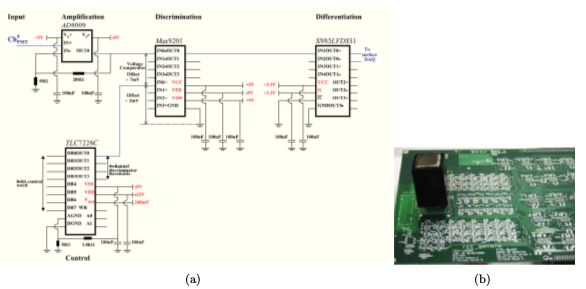
\includegraphics[scale=0.6]{fig5}
 \caption{(a) Diagramas de canales de front-end, exceptuando el amplificador, cada 
 dispositivo controla 4 canales. Entonces en una tarjeta de front-end existen 16 de esos 
 componentes y 64 amplificadores. (b) Vista general de la tarjeta de frond end 
 con el tubo fotomultiplicador multiánodo. Tomada de \cite{trovato}.}
\end{figure}

\subsection{Tubo fotomultiplicador}

BATATA usa fotomultiplicadores multiánodos Hamamatsu H7546B. Las principales características 
de estos dispositivos son:

\begin{itemize}
 \item $8 \times 8$ con un tamaño de ánodo 2 mm $\times$ 2mm.
 \item Área efectiva de 18.1 mm $\times$ 18.1 mm.
 \item Respuesta de alta velocidad.
 \item Bajo cross-talk (2\% típicamente).
 \item Alta sensitividad del cátodo.
\end{itemize}



\section{Críticas y propuestas al detector}

\subsection{Geometría del detector}

\subsection{El centellador}

\subsection{Fibra óptica}

\subsection{Electrónica}

\subsection{Tubo fotomultiplicador}

\section*{Conclusiones}

\begin{thebibliography}{10}
 \bibitem{alfaro}
 R. Alfaro et al., \emph{Buried plastic scintillator muon telescope (BATATA)}, 
 Nuclear Instruments and Methods in Physics Research, vol. 617, pp. 511-514, 2010.
 \bibitem{trovato}
 E. Trovato, \emph{Perfomance study of the muon prototype detector at the Pierre 
 Auger Observatory}, Tesis de Doctorado, Università Degli Studi Di Catania, 2011.
 \bibitem{minos}
 The MINOS Collaboration, \emph{MINOS Technical Desing Report}, Documento interno 
 FNAL, NuMI-L-337, 1998. 
\end{thebibliography}


\end{document}